\documentclass[12pt,a4paper,openany,tikz]{book}

\usepackage[utf8]{inputenc}
\usepackage{cmap}
\usepackage{type1ec}
\usepackage[T1]{fontenc}
\usepackage{fancyhdr}
\usepackage{graphicx,epsfig}
\usepackage[slovene]{babel}
\usepackage{cite}
\usepackage{mathrsfs}
\usepackage{enumitem}
\usepackage{todonotes}
\usepackage{mdframed}
\usepackage{mathtools}
\usepackage{amsmath}
\usepackage{amssymb}
\usepackage{caption}
\usepackage{subcaption}
\usepackage{tikz}
\usetikzlibrary{graphs,graphs.standard,quotes}
\usepackage[a4paper, headheight=15pt]{geometry}
\renewcommand{\baselinestretch}{1.3}



\usepackage[pdftex,colorlinks,citecolor=black,filecolor=black,linkcolor=black,urlcolor=black,pagebackref,unicode]{hyperref}
\usepackage[acronym,toc,xindy]{glossaries}
\usepackage{tikz}

%Nastavitev glave in repa strani
\pagestyle{fancy}
\fancyhead{}
\renewcommand{\chaptermark}[1]{\markboth{\textsf{Poglavje \thechapter:\ #1}}{}}
\renewcommand{\sectionmark}[1]{\markright{\textsf{\thesection\  #1}}{}}
\fancyhead[RE]{\leftmark}
\fancyhead[LO]{\rightmark}
\fancyhead[LE,RO]{\thepage}
\fancyfoot{}
\renewcommand{\headrulewidth}{0.0pt}
\renewcommand{\footrulewidth}{0.0pt}

\newcommand{\gnuplot}{\textbf{gnuplot}}
\newcommand{\pgfname}{\textsc{pgf}}
\newcommand{\tikzname}{Ti\emph{k}Z}

\DeclareMathAlphabet{\mathpzc}{OT1}{pzc}{m}{it}
\mdfsetup{nobreak=true}
\makeglossaries{}
%%%%%%%%%%%%%%%%%%%%%%%%%%%%%%%%%%%%%%%%%%%%%%%%%%%%%%%%%%%%%%%%
%% ccBeamer 0.1, 2007-07-02                                   %%
%% Written by Sebastian Pipping <webmaster@hartwork.org>      %%
%% ---------------------------------------------------------- %%
%% Licensed under Creative Commons Attribution-ShareAlike 3.0 %%
%% http://creativecommons.org/licenses/by-sa/3.0/             %%
%%%%%%%%%%%%%%%%%%%%%%%%%%%%%%%%%%%%%%%%%%%%%%%%%%%%%%%%%%%%%%%%


%% Images
\newcommand{\CcImageBy}[1]{%
	
\includegraphics[scale=#1]{creative_commons/cc_by_30.pdf}%
}
\newcommand{\CcImageCc}[1]{%
	
\includegraphics[scale=#1]{creative_commons/cc_cc_30.pdf}%
}
\newcommand{\CcImageDevNations}[1]{%
	
\includegraphics[scale=#1]{creative_commons/cc_dev_nations_30.pdf}%
}
\newcommand{\CcImageNc}[1]{%
	
\includegraphics[scale=#1]{creative_commons/cc_nc_30.pdf}%
}
\newcommand{\CcImageNd}[1]{%
	
\includegraphics[scale=#1]{creative_commons/cc_nd_30.pdf}%
}
\newcommand{\CcImagePd}[1]{%
	
\includegraphics[scale=#1]{creative_commons/cc_pd_30.pdf}%
}
\newcommand{\CcImageSa}[1]{%
	
\includegraphics[scale=#1]{creative_commons/cc_sa_30.pdf}%
}
\newcommand{\CcImageSampling}[1]{%
	
\includegraphics[scale=#1]{creative_commons/cc_sampling_30.pdf}%
}
\newcommand{\CcImageSamplingPlus}[1]{%
	
\includegraphics[scale=#1]{creative_commons/cc_sampling_plus_30.pdf}%
}


%% Groups
\newcommand{\CcGroupBy}[1]{% zoom
	\CcImageBy{#1}%
}
\newcommand{\CcGroupByNc}[2]{% zoom, gap
	\CcImageBy{#1}\hspace*{#2}\CcImageNc{#1}%
}
\newcommand{\CcGroupByNcNd}[2]{% zoom, gap
	\CcImageBy{#1}\hspace*{#2}\CcImageNc{#1}\hspace*{#2}\CcImageNd{#1}%
}
\newcommand{\CcGroupByNcSa}[2]{% zoom, gap
	\CcImageBy{#1}\hspace*{#2}\CcImageNc{#1}\hspace*{#2}\CcImageSa{#1}%
}
\newcommand{\CcGroupByNd}[2]{% zoom, gap
	\CcImageBy{#1}\hspace*{#2}\CcImageNd{#1}%
}
\newcommand{\CcGroupBySa}[2]{% zoom, gap
	\CcImageBy{#1}\hspace*{#2}\CcImageSa{#1}%
}
\newcommand{\CcGroupDevNations}[1]{% zoom
	\CcImageDevNations{#1}%
}
\newcommand{\CcGroupNcSampling}[2]{% zoom, gap
	\CcImageNc{#1}\hspace*{#2}\CcImageSampling{#1}%
}
\newcommand{\CcGroupPd}[1]{% zoom
	\CcImagePd{#1}%
}
\newcommand{\CcGroupSampling}[1]{% zoom
	\CcImageSampling{#1}%
}
\newcommand{\CcGroupSamplingPlus}[1]{% zoom
	\CcImageSamplingPlus{#1}%
}


%********************************************

\begin{document}

% stran 1 med uvodnimi listi
\thispagestyle{empty}

\begin{center}
{\large
UNIVERZA V LJUBLJANI\\
FAKULTETA ZA RAČUNALNIŠTVO IN INFORMATIKO\\
}

\vspace{3cm}
{\LARGE Andraž Vrhovec}\\

\vspace{2cm}
\textsc{\textbf{\LARGE
Varnost podatkov v oblaku
}}

\vspace{2cm}
{ DIPLOMSKO DELO}\\
{ NA INTERDISCIPLINARNEM UNIVERZITETNEM ŠTUDIJU
}


\vspace{2cm}
{\Large Mentor: prof.\ dr.\ Aleksandar Jurišić}

\vfill
{\Large Ljubljana, 2016}
\end{center}

\newpage

\ \thispagestyle{empty}

\newpage

%********************************************

% stran 2 med uvodnimi listi
\thispagestyle{empty}

\vspace*{5cm}
{\small \noindent
To diplomsko delo je ponujeno pod licenco \textit{Creative Commons Priznanje avtorstva-Deljenje pod enakimi pogoji 2.5 Slovenija}
ali (po želji) novejšo različico.
To pomeni, da se tako besedilo, slike, grafi in druge sestavine dela kot tudi rezultati diplomskega dela lahko prosto distribuirajo,
reproducirajo, uporabljajo, dajejo v najem, priobčujejo javnosti in predelujejo, pod pogojem, da se jasno in vidno navede avtorja in naslov tega
dela in da se v primeru spremembe, preoblikovanja ali uporabe tega dela v svojem delu, lahko distribuira predelava le pod
licenco, ki je enaka tej.
Podrobnosti licence so dostopne na spletni strani \url{http://creativecommons.si/} ali na Inštitutu za
intelektualno lastnino, Streliška 1, 1000 Ljubljana.

\begin{center}% 0.66 / 0.89 = 0.741573033707865
  \CcImageCc{0.741573033707865}\hspace*{1ex}\CcGroupBySa{1}{1ex}
\end{center}
}

\begin{center}
\vfill
{\em
Besedilo je oblikovano z urejevalnikom besedil \LaTeX.
}
\end{center}

\newpage

\ \thispagestyle{empty}

\newpage

%********************************************

% stran 3 med uvodnimi listi
\thispagestyle{empty}

Namesto te strani {\bf vstavite} original izdane teme diplomskega dela s podpisom mentorja in dekana ter žigom fakultete, ki ga diplomant
dvigne v študentskem referatu, preden odda izdelek v vezavo!

\newpage

%********************************************

% stran 4 med uvodnimi listi je prazna
\ \thispagestyle{empty}

\newpage

%********************************************

% stran 5 med uvodnimi listi

\thispagestyle{empty}

\vspace{1cm}
\begin{center}
{\Large \textbf{IZJAVA O AVTORSTVU}}
\end{center}

\begin{center}
{\Large diplomskega dela}
\end{center}

\vspace{1cm}
Spodaj podpisani/-a \hspace{0.5cm} Andraž Vrhovec,

\vspace{0.5cm}
z vpisno številko \hspace{0.5cm} 63080117,

\vspace{1cm}
sem avtor diplomskega dela z naslovom:

\vspace{0.5cm}
Varnost v oblaku
\vspace{1.5cm}
S svojim podpisom zagotavljam, da:
\begin{itemize}
	\item sem diplomsko delo izdelal/-a samostojno pod mentorstvom

	prof.\ dr.\ Aleksandar Jurišić

	\item	so elektronska oblika diplomskega dela, naslov (slov., angl.), povzetek (slov., angl.) ter ključne besede (slov., angl.) identični s tiskano obliko diplomskega dela
	\item soglašam z javno objavo elektronske oblike diplomskega dela v zbirki ``Dela FRI''.
\end{itemize}

\vspace{1cm}
V Ljubljani, dne \today \hspace{1cm} Podpis avtorja/-ice:

\newpage

%*******************************************

% stran 6 med uvodnimi listi je prazna pri dvostranskem tiskanju
\ \thispagestyle{empty}

\newpage

%********************************************

% stran 7 med uvodnimi listi

\chapter*{Zahvala}

\thispagestyle{empty}
ablak
Mogoče


\newpage

%********************************************

% stran 8 med uvodnimi listi je prazna pri dvostranskem tiskanju
\ \thispagestyle{empty}

\newpage

%********************************************

% stran 9 med uvodnimi listi
\thispagestyle{empty}

$\;$

\vspace{5cm}
\hfill{\Large \em Morebitno posvetilo\/ }
\thispagestyle{empty}

\newpage

% stran 10 med uvodnimi listi je prazna pri dvostranskem tiskanju

\ \thispagestyle{empty}

\newpage

%********************************************

\renewcommand\thepage{}
\tableofcontents
\renewcommand\thepage{\arabic{page}}

\thispagestyle{empty}


%********************************************

\chapter*{Seznam uporabljenih kratic in simbolov}
\thispagestyle{empty}

\printglossaries{}

%\cleardoublepage

\clearpage{\pagestyle{empty}\cleardoublepage}

%********************************************
%začno se glavni listi, ki so numerirani z arabskimi stevilkami

\setcounter{page}{1}
\pagenumbering{arabic}

\chapter*{Povzetek}

\addcontentsline{toc}{chapter}{Povzetek}

\todo[inline]{Napiši povzetek}

\vspace{1.3cm}
\noindent
{\large \bf Ključne besede:}

\vspace{0.5cm}
\noindent
diploma, oblak, varnost, kriptografija


\chapter*{Abstract}

\addcontentsline{toc}{chapter}{Abstract}

Povzetek naj bo napisan v angleškem jeziku.

\vspace{1.3cm}
\noindent
{\large \bf Key words:}

\vspace{0.5cm}
\noindent
Ključne besede v angleškem jeziku.


%********************************************

\chapter{Uvod}

V zadnjih letih smo priča bliskovitemu porastu popularnosti tako imenovanega računalništva v oblaku. Gartner je v začetku leta 2015 uvrstil računalništvo v oblaku med 10 strateško najpomembnejših tehnoloških trendov, ki bodo krojili prihodnost. Oblak nam omogoča udobno, cenovno ugodno delo, kadarkoli in kjerkoli, tudi zunaj pisarne, saj je vse kar potrebujemo internetni dostop in računalnik ali telefon. Računalništvo v oblaku je posledica razvoja več različnih tehnologij, ki so skupaj omogočile cenovno učinkovite rešitve, ki so hkrati preproste za uporabo. Končni uporabniki uporabljajo oblak, ker je preprosto za uporabo, omogoča dostop do podatkov kjerkoli in kadarkoli. Na drugi strani vedno več podjetji v žeji, da znižajo stroške poslovanja in povečajo sposobnost prilagajanja zahtevam trga, seli svoje poslovanje v oblak. Posledica tega premika je selitev podatkov iz fizičnih nosilcev, ki so bili tradicionalno v lasti iste osebe kot podatki, v oblak. To pomeni da varnost hrambe svojih podatkov zaupamo tretjim osebam, kar niti ni nujno tako slabo, kot se sliši. Za veliko ljudi in manjših podjetji je skrb za varnost podatkov velik zalogaj, ki zahteva ustrezno tehnično izobrazbo, strojno opremo in prostor. Kadar hranimo podatke v oblaku, nič od tega ni potrebno, saj nam vse to zagotavlja ponudnik storitev v oblaku v zameno za mesečno naročnino. V nadaljevanju tega dela, bomo najprej pregledali kaj je oblak, kakšne oblike oblaka poznamo. Ko bomo opremljeni z osnovnim poznavanjem oblaka, si bomo pogledali še formalno definicijo varnosti nato pa bomo preučili kako vpeljava in vsesplošna uporaba oblaka vpliva na varnost naših podatkov.


\section{Kaj je oblak?}
\label{sec:Kaj je oblak?}


Priljubljen internetni rek gre nekako takole: “There is no cloud, just someone else's computer”. Preprosto rečeno je to delno res, saj oblak ni nič drugega kot skupek velikega števila računalnikov, ki niso v lasti uporabnika storitve v oblaku, morda niso niti v lasti ponudnika storitve, ampak jih ta najema pri tretjem ponudniku. Pojem oblak je le krovni izraz za nove načine ponudbe in uporabe storitev, zato ga moramo podrobneje razdelati in razložiti.

NIST opredeli oblak kot: ``Računalništvo v oblaku je model, ki omogoča vseprisoten preprost dostop na zahtevo do skupnega računalniških virov (omrežja, strežniki, pomnilniški mediji, aplikacije in storitve), ki so lahko hitro pridobljeni ali sproščeni z minimalnim trudom in popolnoma samodejno, brez posredovanja ponudnika storitve. Model oblaka sestavlja pet ključnih lastnosti, trije nivoji storitve in štirje tipi oblakov.''~\cite{mell2011nist}

\begin{description}[style=nextline]
   \item[Storitev na zahtevo] Stranka lahko pridobi nove vire v oblaku po potrebi, lahko tudi popolnoma samodejno brez človeškega posredovanja.

   \item[Širok dostop preko omrežja] Zmogljivosti oblaka so na voljo preko omrežja in do njih lahko dostopamo preko standardnih mehanizmov, kar omogoča dostop praktično katerekoli naprave, ki se je zmožna povezati v omrežje (telefoni, tablice, računalniki, …).

   \item[Uporaba skupnih virov] Ponudnikovi fizični viri so združeni v bazen virov iz katerega stranke dobijo virtualizirane vire. Virtualizirani vir lahko prosto prehaja med fizičnimi gostitelji, zato težko govorimo o točni lokaciji vira.

   \item[Bliskovita prožnost] Uporabnik lahko preprosto poveča ali zmanjša zmogljivosti virov, ki jih potrebuje glede na potrebe. Uporabnik ima pogosto občutek da so mu na voljo neomejene zmogljivosti.

   \item[Merjenje porabe in obračun glede na porabo virov]  Oblačni sistemi samodejno nadzirajo in optimizirajo porabo virov s pomočjo metrik (poraba prostora, pasovne širine, procesorskega časa \ldots). Poraba virov se nadzira, kontrolira in poroča, kar omogoča transparentnost za ponudnika in uporabnika.
\end{description}

\newacronym{SaaS}{SaaS}{Software as a Service}
\newacronym{PaaS}{PaaS}{Platform as a Service}
\newacronym{IaaS}{IaaS}{Infrastructure as a Service}
\newacronym{API}{API}{Application programming interface}

\begin{description}[style=nextline]
	\item[\gls{SaaS}] Ponudnik storitev uporabniku omogoča uporabo njegove aplikacije, ki teče v oblaku. Aplikacija je dosegljiva iz različnih naprav, preko recimo spletnega brskalnika ali aplikacijskega vmesnika (\gls{API}). Uporabnik nima nadzora nad infrastrukturo na kateri teče aplikacija (omrežje in strežniki), kot tudi ne nad samo aplikacijo (z izjemo konfiguracije aplikacije).

	\item[\gls{PaaS}]: Ponudnik storitev uporabniku ponuja platformo, na katero lahko uporabnik namesti lastne ali kupljene aplikacije, ki so prilagojene za delovanje v oblaku. Tudi tu uporabnik nima nadzora nad infrastrukturo na kateri teče aplikacije, ima pa popolni nadzor nad aplikacijo.

	\item[\gls{IaaS}]: Ponudnik uporabniku omogoča postavitev osnovnih gradnikov računalniškega sistema (procesiranje, hramba podatkov, omrežje …) iz katerih lahko uporabnik sestavi kar želi. Uporabnik sicer nima nadzora nad spodaj ležečo fizično infrastrukturo, vendar ima ves nadzor nad virtualiziranimi viri ki jih pridobi.
\end{description}

\begin{description}[style=nextline]
	\item[Zasebni oblak] Vsa infrastruktura je namenjena uporabi znotraj ene organizacije, ki je sestavljena iz več delov. Upravljanje, vzdrževanje in lastništvo je lahko v domeni iste organizacije, tretje osebe ali kombinacije obojega. Lokacija sistema je lahko v prostorih organizacije ali pa izven.

	\item[Skupni oblak] Infrastruktura je namenjena uporabi s strani skupnosti organizacij, ki imajo skupne zahteve ali skupni cilj. Upravljanje, vzdrževanje in lastništvo je lahko v domeni ene ali večih organizacij znotraj skupnosti, tretje osebe ali kombinacije obojega. Lokacija sistema je lahko v prostorih ene od organizacij ali pa izven.

	\item[Javni oblak] Infrastruktura je namenjena uporabi s strani vseh. Ponudnik je lahko zasebno podjetje, izobraževalna ustanova ali vladna agencija. Infrastruktura se ponavadi nahaja na lokaciji ponudnika.
	Hibridni oblak: Hibridni oblak je kombinacija dveh ali več tipov oblakov iz prvih treh točk (zasebni, javni, skupni). Oblaka sta sicer fizično ločena, vendar skupni standardi in tehnologije omogočajo preprosto prehajanje aplikacij in podatkov iz enega na drugega.
\end{description}

\section{Kaj je varnost?}
Varnost je širok pojem, ki ga v kontekstu računalništva lahko razdelimo na tri dele. To so: računalniška varnost (computer security), informacijska varnost (information security) in varovanje podatkov (information assurance).

\newglossaryentry{neizpodbitnost}
{
  name=preprečevanje tajenja,
  description={non-repudiation},
}

\begin{description}

	\item[Računalniška varnost] se ukvarja z varovanjem računalniških sistemov, od strojne opreme preko programske opreme do podatkov, ki se procesirajo na tej strojni opremi. Naloga računalniške varnosti je zagotoviti integriteto, dostopnost in zaupnost vseh sestavnih delov računalniškega sistema.

\item[Informacijska varnost] se ukvarja z varovanjem podatkov, ki se obdelujejo in shranjujejo v informacijskih sistemih. Njena naloga je zaščititi podatke pred nepooblaščenim dostopom, uporabo, spreminjanjem in uničenjem z ciljem zagotavljanja integritete, dostopnosti in zaupnosti podatkov.

\item[Varovanje podatkov] se ukvarja z varovanjem podatkov in upravljanjem tveganj povezanih z uporabo, prenosom in procesiranjem podatkov z ciljem zagotavljanja integritete, dostopnosti, zaupnosti in neizpodbitnostjo podatkov.
\end{description}

Iz teh opisov lahko razberemo ključne lastnosti varnega računalniškega sistema. V literaturi se te ključne tri lastnosti imenujemo CIA triad, kjer je CIA angleška kratica za ključne 3 lastnosti:

\newglossaryentry{zaupnost}
{
  name=zaupnost,
  description={Confidentiality},
}

\newglossaryentry{celovitost}
{
  name=celovitost,
  description={Integrity},
}

\newglossaryentry{razpolozljivost}
{
  name=razpoložljivost,
  description={Availability},
}

\begin{description}
\item[\Gls{zaupnost}] pomeni zasebnost podatkov. Ukrepi, ki zagotavljajo zaupnost podatkov so usmerjeni k preprečevanju dostopa nepooblaščenih oseb. Pogosti mehanizmi, ki se uporabljajo za zagotavljanje zaupnosti podatkov so zaščita z uporabniškim imenom in geslom, dvostopenjska overitev (two-factor auth), biometrična overitev in šifriranje podatkov.

\item[\Gls{celovitost}] pomeni ohranjanje točnosti in pravilnosti podatkov. Ukrepi, ki zagotavljajo celovitost podatkov, preprečujejo nepooblaščenim osebam spreminjanje podatkov med prenosom ali v mirovanju. Omogočajo sledenje spremembam podatkov skozi zgodovino (revizijska sled), obnovitev podatkov iz varnostne kopije v primeru da pride do nepooblaščene spremembe. Mehanizmi, ki zagotavljajo celovitost podatkov so nadzor dostopa in zgoščevalne funkcije in digitalni podpisi.

\item[\Gls{razpolozljivost}] pomeni da so podatki vedno na voljo pooblaščenim osebam. Glavni vzrok nerazpoložljivosti so programske in strojne napake ter napadi zavrnitve storitve (denial of service). Razpoložljivost podatkov se zagotavlja z rednim vzdrževanjem strojne in programske opreme in s posebnimi ukrepi za preprečevanje napadov zavrnitve storitve.

\end{description}

Poleg treh ključnih lastnosti, ki jih najdemo zgoraj je Meier identificiral še tri lastnosti, to so:

\newglossaryentry{overjanje}
{
  name=overjanje,
  description={Authentication},
}

\newglossaryentry{avtorizacija}
{
  name=avtorizacija,
  description={Authorization},
}

\newglossaryentry{neizpodbitnost}
{
  name=neizpodbitnost,
  description={Non-repudioation},
}

\begin{description}

\item[\Gls{overjanje}] identificira vir podatka oziroma izvor operacije, ki je lahko človek ali računalnik in se prepričamo da je res tisti za katerega se izdaja.

\item[\Gls{avtorizacija}] nadzira dostop do virov glede na pravila sistema in dodeljene pravice. Avtorizacijski mehanizmi uporabnikom preprečujejo da bi presegli svoja pooblastila.

\item[\Gls{neizpodbitnost}] onemogoča uporabniku da izpodbija oziroma zanika neko dejanje ali veljavnost pogodbe.

\end{description}

Vse zgoraj naštete lastnosti so splošne lastnosti varnosti in se kot take seveda tičejo tudi računalništva v oblaku. Pri uporabi storitev v oblaku bi morali najbolj izpostaviti vprašanje varnosti podatkov, saj le te zaupamo v hrambo ponudniku storitve.

\chapter{Varnostna tveganja v oblaku}

Zaradi vse večje popularnosti storitev v oblaku in posledično ogromne količine podatkov, s katerimi razpolagajo ponudniki storitev v oblaku, so ti vedno pogosteje tarča napadov kriminalnih združb. Za sisteme, ki tečejo “v oblaku”, je značilno da navzven delujejo kot en strežnik, v resnici pa tečejo na velikem številu strežnikov, ki so med seboj povezani. To pomeni da morebitni vdor v samo en strežnik napadalcu omogoča dostop tudi na druge strežnike, ki tečejo znotraj istega sistema. Če si sistem predstavljamo kot trdnjavo, to pomeni da je večina zaščitnih mehanizmov skoncentrirana na obrobju, na obzidju trdnjave. Če uspemo to obzidje predreti na samo enem delčku, se potem lahko več ali manj prosto sprehajamo znotraj trdnjave. Pred pojavom storitev v oblaku je bilo znotraj enega obzidja le nekaj strežnikov, zato je bilo obzidje malo in ga je bilo lažje vzdrževati. Sistem, na katerem teče storitev v oblaku pa je lahko sestavljen iz več tisoč strežnikov, kar pomeni da velikost obzidja močno poveča in veliko obzidje je težko vzdrževati, zato se kaj hitro v njem pojavijo razpoke.

Druga stvar, ki dela sisteme v oblaku zanimive za napadalce je koncentracija podatkov. V primeru do vdora v klasični strežnik, napadalec dobi dostop do veliko manjše količine podatkov kot ob vdoru v oblačni sistem. Razlog je preprost, saj na en sam strežnik fizično ni mogoče shraniti toliko podatkov, kot na sistem, ki je sestavljen iz tičoče strežnikov.

Ranljivost računalniškega sistema je lastnost, zaradi katere je ogroženo njegovo delovanje in varnost podatkov, ki jih vsebuje. Storitve, ki delujejo v oblaku tako podedujejo vse ranljivosti, ki jih imajo klasični računalniški sistemi, zaradi posebnih lastnosti oblaka, pa obstaja se nekaj groženj, specifičnih za storitve v oblaku:

\newglossaryentry{MITM}
{
  name={napad vrinjenega napadalca},
  description={angl.\ man-in-the-middle/MITM attack}
}

\begin{description}[style=nextline]

\item[Nedovoljen dostop do upraviteljskega in programskega vmesnika] Narava storitev v oblaku zahteva da so upraviteljski vmesniki dostopni preko Interneta široki množici uporabnikov, kar posledično pomeni da so ti vmesniki izpostavljeni napadom preko Interneta.

\item[Ranljivosti internetnega protokola] Ena ključnih lastnosti oblaka je tudi široka dostopnost preko standardiziranih protokolov kot je Internetni protokol, zato je potrebno ko govorimo o varnosti v oblaku upoštevati tudi vse ranljivosti Internetnega protokola, kot je recimo \gls{MITM}.

\item[Ranljivosti obnovitve podatkov] Zaradi uporabe skupnih virov, ki je ena ključnih lastnosti oblaka, se lahko en fizični nosilec podatkov, ki je prej pripadal enemu uporabniku kasneje dodeli drugemu uporabniku. Če pred tem ne poskrbimo za varen izbris podatkov, lahko drugi uporabnik obnovi izbrisane podatke z nosilca in tako pride do razkritja podatkov.

\item[Izogibanje merjenju in plačilu] Storitve v oblaku se običajno plačujejo po porabi. Prav tako, da pričnemo uporabljati storitev praviloma potrebujemo vnesti samo nekaj osnovnih podatkov in številko kreditne kartice. Napadalec nam lahko predloži ukradene podatke ali manipulira podatke o porabi, tako da se izogne plačilu.

\end{description}

\section{Izzivi na področju varnosti v oblaku}
\label{sec:Izzivi na področju varnosti v oblaku}


\subsection{Razkritje podatkov}
\label{sub:Razkritje podatkov}

O razkritju podatkov govorimo v primeru, da se občutljivi in zaupni podatki znajdejo na očeh nepooblaščenih oseb ali javnosti.  To se lahko zgodi kot posledica usmerjenega napada ali preprosto zaradi človeške napake, napake v aplikaciji ali slabih varnostnih mehanizmov aplikacije. Primeri zaupnih podatkov, ki so pogosto tarča napadov so: zdravstveni podatki, finančni podatki, osebno določljivi podatki, poslovne skrivnosti in intelektualna lastnina.

Razkritje podatkov je stara in vseprisotna grožnja v vseh računalniških sistemih, vendar zaradi prej omenjene koncentracije podatkov je ta grožnja v oblačnih sistemih še večja.

Obseg škode, ki ga povzroči razkritje podatkov je odvisen od občutljivosti podatkov, ki so bili odtujeni. V veliko državah po svetu obstajajo zakoni in predpisi, ki podjetja ki hranijo določene tipe občutljivih podatkov obvezuje k določenim standardom zaščite. V primeru, da pride do razkritja podatkov, lahko odgovorno podjetje doleti denarna kazen ali celo kazenska ovadba. Poleg škode, ki je bila povzročena z razkritjem podatkov in morebitno denarno kaznijo so tu še stroški preiskave incidenta, obveščanja uporabnikov in izguba ugleda podjetja.

\subsection{Pomanjkljivo upravljanje identitete, poverilnic in nadzora dostopa}
\label{sub:Pomanjkljivo upravljanje identitete, poverilnic in nadzora dostopa}

Površno upravljanje lahko pripelje do nenamernega razkritja uporabniških imen, gesel in ključev, ki se uporabljajo za dostop do storitev. Ponudniki storitev v oblaku upravljajo z identitetami milijonov uporabnikov in zaposlenimi, zato je potrebna velika skrb da se zagotovi pravilno uupravljanje identitete skozi celoten cikel. Potrebno je poskrbeti za takojšno prekinitev veljavnosti identitete, v primeru da pride do odpovedi delovnega razmerja zaposlenega ali prekinitve pogodbe s stranko. Uporaba šibkih gesel in neuporaba dvostopenjske avtentikacije in neuporaba rotacije šifrirnih ključev, gesel in certifikatov so primeri slabe prakse, ki v primeru napada napadalcu olajšajodelo in povečajo razsežnosti škode, ki jo napadalec lahko povzroči.

\subsection{Nezaščiteni uporabniški in programski vmesniki}
\label{sub:Nezaščiteni uporabniški in programski vmesniki}

Ponudniki storitev v oblaku ponujajo nabor uporabniški in programskih vmesnikov, preko katerih uporabniki dostopajo do storitev ponudnika. So stična točka med uporabnikom in storitvijo in od varnosti in dostopnosti teh vmesnikov je odvisna varnost celotnega sistema. So prva linija obrambe sistema, zato je pri zasnovi teh vmesnikov potrebno misliti na varnost s pravilno implementacijo varnostnih mehanizmov kot so avtentikacija, nadzor dostopa in šifriranje. Vmesniki morajo biti zasnovani tako, da ščitijo pred namerno in nenamerno zlorabo sistema.

\subsection{Sistemske ranljivosti}
\label{sub:Sistemske ranljivosti}

Sistemske ranljivosti so preprosto povedano hrošči v uporabljeni programski opremi, katere je možno izkoristiti za napad na računalniški sistem. Ranljivosti, ki se nahajajo v jedru operacijskega sistema ali sistemskih knjižnicah predstavljajo grožnjo za celoten sistem.

Tako kot večina ostalih predstavljenih groženj, tudi sistemske ranljivosti niso nič novega, vendar razsežnost oblačnih sistemov doda takim ranljivostim popolnoma nov pomen. Zaradi napredka tehnologije je možno na enem strežniku gostiti več virtualnih strežnikov različnih organizacij, kar pomeni da si ti virtualni strežniki delijo pomnilnik in ostale vire, kar omogoča nove načine izrabe sistemskih ranljivosti.

\subsection{Ugrabitev uporabniškega računa}
\label{sub:Ugrabitev uporabniškega računa}

Ugrabitve uporabniških računov so posledica napadov ribarjenja, prevare ali izkoriščanja sistemskih pomanjkljivosti. V primeru, da ista uporabniška imena in gesla uporabljamo za več različnih storitev, to še dodatno poveča posledice napada. V primeru, da pride do ugrabitve uporabniškega računa za storitev v oblaku, lahko napadalec izkoristi to storitev kot odskočno desko za nove napade.

\subsection{Notranje grožnje}
\label{sub:Notranje grožnje}

Tveganje, ki ga predstavljajo notranje grožnje, kot so škodoželjni zaposleni, je dokaj novo in še vedno predmet debate v industriji računalniške varnosti. Dejstvo je da tako tveganje obstaja, predvsem pri uporabi javnega oblaka, saj v tem primeru z infrastrukturo in podatki razpolaga tretja oseba. V tem primeru uporabnik storitve nima nikakršnega mehanizma, s katerim bi lahko nadziral zaposlene pri ponudniku storitve.

\subsection{Organizirana trajna grožnja}
\label{sub:Organizirana trajna grožnja}

Organiziranje trajne grožnje so ena najnaprednejših oblik grožnje računalniški varnosti. Za napadi te oblike so ponavadi skrivajo velike organizacije z državno podporo (tajne službe, vojska). Značilnost te oblike napada je, da napadalec temeljito preuči ciljni sistem, njegovo organizacijo in šibke točke. Ta oblika napada se pogosto začne z usmerjenim izvabljanjem, to je posebna tehnika ribarjenja, ki je usmerjena proti točno določenim osebam, v našem primeru zaposleni v ciljni organizaciji. S pomočjo usmerjenega izvabljanja napadalec poskuša pridobiti vstopno točko v ciljni sistem. Ko enkrat pridobi dostop do notranjega omrežja sistema, to uporabi kot odskočno desko za nadaljnje premike proti željenim tarčam. Cilj napada so podatki, ki se nahajajo v sistemu žrtve, pogosto so to poslovne skrivnosti ali državne tajne. Napadalec želi čimdlje ostati skrit, saj tako pridobi dostop do večjega števila računalnikov znotraj omrežja in s tem večje količine podatkov. V želji da ostane skrit, uporablja napredne tehnike brisanja sledov, zato je take tipe napada zelo težko zaznati, saj navzven sistem izgleda kot da deluje normalno.

Posebna oblika organiziranih trajnih groženj so kibernetska orožja. Verjetno najbolj znan med njimi je Stuxnet, ki je sabotiral Iranski jedrski program. Kibernetska orožja se od ostalih oblik napadov razlikujejo v tem, da žrtvi povzročijo dejansko fizično škodo v obliki uničene opreme.

\subsection{Izguba podatkov}
\label{sub:Izguba podatkov}

Izguba podatkov predstavlja za večino uporabnikov in podjetji eno najhujših nočnih mor. Trajna izguba podatkov, shranjenih v oblaku ni nujno posledica napada tretje osebe, ampak je lahko tudi posledica malomarnosti, kot je recimo nenameren izbris podatkov s strani ponudnika storitve ali posledica naravne katastrofe kot je požar ali potres. V izogib trajni izgubi podatkov ponudniki storitev v oblaku uporabljajo različne mehanizme, kot so geografska redundanca in varnostno kopiranje na drugo lokacijo. Vendar v primeru, da uporabnik podatke šifrira še preden jih pošlje oblak in nato izgubi šifrirni ključ, noben od naštetih mehanizmov ne more preprečiti takojšne in trajne izgube podatkov.

\subsection{Malomarnost}
\label{sub:Malomarnost}

Preden začnemo uporabljati storitve v oblaku, je potrebno preučiti vse aspekte, ki jih bo taka sprememba prinesla. Vodilni kadri v podjetjih pogosto nimajo dovolj poglobljenega poznavanja oblaka s tehnološkega vidika, kot tudi ne poznajo pravnih zank, ki jih vsebujejo “pogoji uporabe” določenih ponudnikov storitev v oblaku. V primeru, da pred uporabo storitev v oblaku ne naredimo temeljite analize, lahko pride do tehnoloških, pravnih, skladenjskih in poslovnih tveganj, ki ogrozijo uspeh podjetja.

\subsection{Zloraba in zlonamerna uporaba sistemov}
\label{sub:Zloraba in zlonamerna uporaba sistemov}

Pogosto ponudniki storitev v oblaku omogočajo brezplačne preizkusne račune za omejeno časovno obdobje, pa tudi če jih ne, lahko napadalec s pomočjo ukradenih bančnih podatkov ustvari veliko količino uporabniških računov, ki jih potem izkoristi za izvajanje različnih nelegalnih aktivnosti. Te lažni uporabniški računi napadalcu omogočajo pošiljanje nezaželene pošte, izvajanje napadov ribarjenja ali napadov zavrnitve storitve, ki so lahko usmerjeni k ponudniku storitve, njegovim strankam ali pa tretjim osebam.

\subsection{Napadi zavrnitve storitve}
\label{subs:Napadi zavrnitve storitve}

Napad zavrnitve storitve je ena najpreprostejših in pogosto zelo učinkovitih oblik napada na računalniške sisteme. Cilj napada je uporabnikom preprečiti normalen dostop do storitve, kar napadalec doseže s tem da napaden sistem prisili v nerazumno veliko porabo različnih virov, kot so pasovna širina, procesorski čas ali podatkovni prostor. Najbolj osnovna oblika napada zavrnitve storitve se zanaša na dejstvo da napadalec razpolaga z večjo količino določenega vira (pasovna širina, procesorski čas …) kot napaden sistem. Obstajajo pa tudi bolj prefinjene asimetrične oblike napada, kjer napadalec z veliko manjšo količino virov kot tarča, s pomočjo izrabe varnostne pomanjkljivosti v sistemu ali aplikaciji onemogoči tarčo napada. Napadi zavrnitve storitve običajno ne pustijo trajnih posledic, vendar predstavljajo veliko neprijetnost za uporabnike, saj le ti za čas trajanja napada ne morejo uporabljati storitve, prav tako pa škodujejo ugledu ponudnika.

\subsection{Ranljivosti zaradi uporabe skupnih virov}
\label{sub:Ranljivosti zaradi uporabe skupnih virov}

Zadnji sklop varnostnih groženj v oblaku predstavljajo ranljivosti, ki so posledica ene od ključnih lastnosti oblaka, to je uporaba skupnih virov. Ponudniki storitev v oblaku zagotavljajo navidezno neomejene vire končnemu uporabniku s pomočjo tehnologij virtualizacije in skupne uporabe. Pri tem uporabljajo klasično strojno opremo, ki sicer s pomočjo posebne programske opreme omogoča delitev virov, vendar ni bila zasnovana, da bi omogočala varno skupno uporabo. Tak tip napadov izkorišča dejstvo, da si različni virtualni strežniki delijo fizično strojno opremo, zato je možno s posebno obliko napada, ki se imenuje napad preko stranskega kanala pridobiti informacije iz žrtvinega strežnika, brez da bi dejansko prišlo do vdora. V času pisanja še ni prišlo do takega tipa vdora v praksi, vendar obstajajo primeri takih napadov, ki so jih demonstrirali pod laboratorijskimi pogoji.


\newglossaryentry{plaintext}
{
  name=čistopis,
  description={plaintext},
}


\newglossaryentry{tajnopis}
{
  name=tajnopis,
  description={ciphertext},
}

\newglossaryentry{sifrirnikljuc}
{
  name=šifrirni ključ,
  description={encryption key},
}

\newglossaryentry{otp}
{
  name=enkratni ščit,
  description={(angl.\ one time pad)},
}

\chapter{Zaščita podatkov s pomočjo kriptografije}

Kriptografija omogoča doseganje informacijske varnosti s pomočjo matematičnih postopkov. Verjetno najbolj poznan tak postopek je šifriranje, ki zagotavlja zaupnost podatkov, pogled tega v področje kriptografije spadajo tudi digitalni podpisi, avtentikacijske kode MAC in zgoščevalne funkcije, ki nam pomagajo pri ohranjanju celovitosti in overjanju identitete podatkov.

Šifriranje je način, kako skriti vsebino sporočila (\gls{plaintext}a) pred nepooblaščenimi očmi. To se doseže z uporabo algoritma, ki mu kot vhodni podatek damo \gls{plaintext} in \gls{sifrirnikljuc}, on pa nam vrne \gls{tajnopis}. \Gls{tajnopis} vsebuje enake informacije kot \gls{plaintext}, vendar ima to lastnost, da ga je mogoče prebrati le v primeru, da posedujete ključ za dešifriranje. V kolikor takega ključa ne posedujete, je iz \gls{tajnopis}a praktično nemogoče razbrati vsebino originalnega sporočila.\footnote{Težanost je odvisna od moči kriptografske sheme in pravilnosti implementacije}

To pomeni, da lahko tajnopis javno objavimo, varovati je potrebno samo ključ, s katerim se le ta dešifrira. Ta lastnost nam omogoča, da varno poslujemo s svojo banko, pošiljamo e-pošto, ki jo lahko prebere samo prejemnik navkljub temu, da Internet ni varen komunikacijski kanal in na njemu mrgoli zlobnežev, ki želijo priti do naših zaupnih podatkov.

Potrebno se je zavedati da so formalne zahteve za $100\%$ varnost zelo visoke, zato se v praksi največkrat uporabi princip računske varnosti, ker pomeni da varnost kriptosistema sloni na predpostavi, da so računske zahteve za razbitje kriptografske sheme veliko višje od tistih, ki jih ima na voljo potencialni napadalec. Najbolj znana implementacija popolne varnosti je sicer \gls{otp}, ki ga je leta 1918 patentiral Gilbert S. Vernam~\cite{vernam1919secret}, za katerega je Claude Shannon v leta 1949 objavljenem poročilu\cite{shannon1949communication} dokazal, da zagotavlja popolno varnost. Kot zanimivost lahko povemo, da je domnevno do enakih zaključkov še nekaj let prej, prišel tudi ruski znanstvenik Vladimir Kotelnikov, vendar njegovo poročilo še vedno ostaja zaupno. Problem \glslink{otp}{enkratnega ščita} je v tem, da zahteva ključ enake dolžine kot sporočilo, ki ga želimo šifrirati. Prav tako pa lahko vsak ključ uporabimo samo enkrat, v nasprotnem primeru pa sistem ne zagotavlja več popolne varnosti.

\

Da nam bo lažje, najprej definirajmo kaj je kriptografska shema ali kriptosistem.

\begin{mdframed}[frametitle={Kriptografska shema}]
Kriptografska shema je peterka  $(\mathcal{P}, \mathcal{C}, \mathcal{K},  \mathcal{E}, \mathcal{D})$, kjer veljajo naslednje lastnosti:
	\begin{enumerate}
		\item $\mathcal{P}$ je končna množica možnih čistopisov
		\item $\mathcal{C}$ je končna množica možnih tajnopisov
		\item $\mathcal{K}$ je končna množica možnih ključev
		\item Ta vsak $K \in \mathcal{K}$ obstaja šifrirni postopek $e_K \in \mathcal{E}$ in pripadajoč dešifrirni postopek $d_K \in \mathcal{D}$. Za funkciji $e_K: \mathcal{P} \rightarrow \mathcal{C}$ in $d_K: \mathcal{C} \rightarrow \mathcal{P}$ velja $d_k(e_k(x)) = x$ za vsak $x \in \mathcal{P}$.
	\end{enumerate}
\end{mdframed}

Zgornjo matematično definicijo se da povzeti z naslednjimi besedami. Kriptografsko shemo sestavlja pet sestavin. Čistopisi, tajnopisi, ključi, šifrirni in de-šifrirni postopek. Pomembno je, da ob danem ključu in šifrirnem postopku, obstaja de-šifrirni postopek, ki nam vsak tajnopis, ki je bil šifriran z izbranim šifrirnim postopkom nedvoumno pretvori nazaj v čistopis.

Skozi zgodovino človeštva se je že zelo zgodaj pojavila želja po skrivanju sporočil in s tem so se razvile tudi prve metode šifriranja, vendar nobena od njih ni prestala preizkusa časa.

\

Šifrirne algoritme delimo na dve skupini:
\begin{enumerate}

	\item Simetrične oziroma klasične šifre
	\item Asimetrične šifre oziroma kriptografija javnih ključev

\end{enumerate}

Simetrične šifre so najstarejša in najbolj razširjena vrsta šifriranja, kamor spadajo tudi vse zgodovinske šifre, ki se ne uporabljajo več. Poglavitna lastnost simetričnih šifer je, da se za šifriranje in dešifriranje uporablja enak ključ. Take šifre so lahko zelo preproste in hitre, vendar se pojavi problem distribucije ključev. Tajnopise lahko prenašamo po nezavarovanih kanalih, kar pa ne velja za ključe. To pomeni da si mora vsak par uporabnikov, če želi med sabo komunicirati v šifrirani obliki, najprej preko varnega kanala izmenjati šifrirni ključ. Število potrebnih izmenjav raste $O(n^2)$ glede na število uporabnikov sistema, in na sliki \ref{fig:symmetricproblem} vidimo, da je že pri dvajsetih uporabnikih število potrebnih izmenjav zelo veliko.

\begin{figure}[ht!]
  \centering
  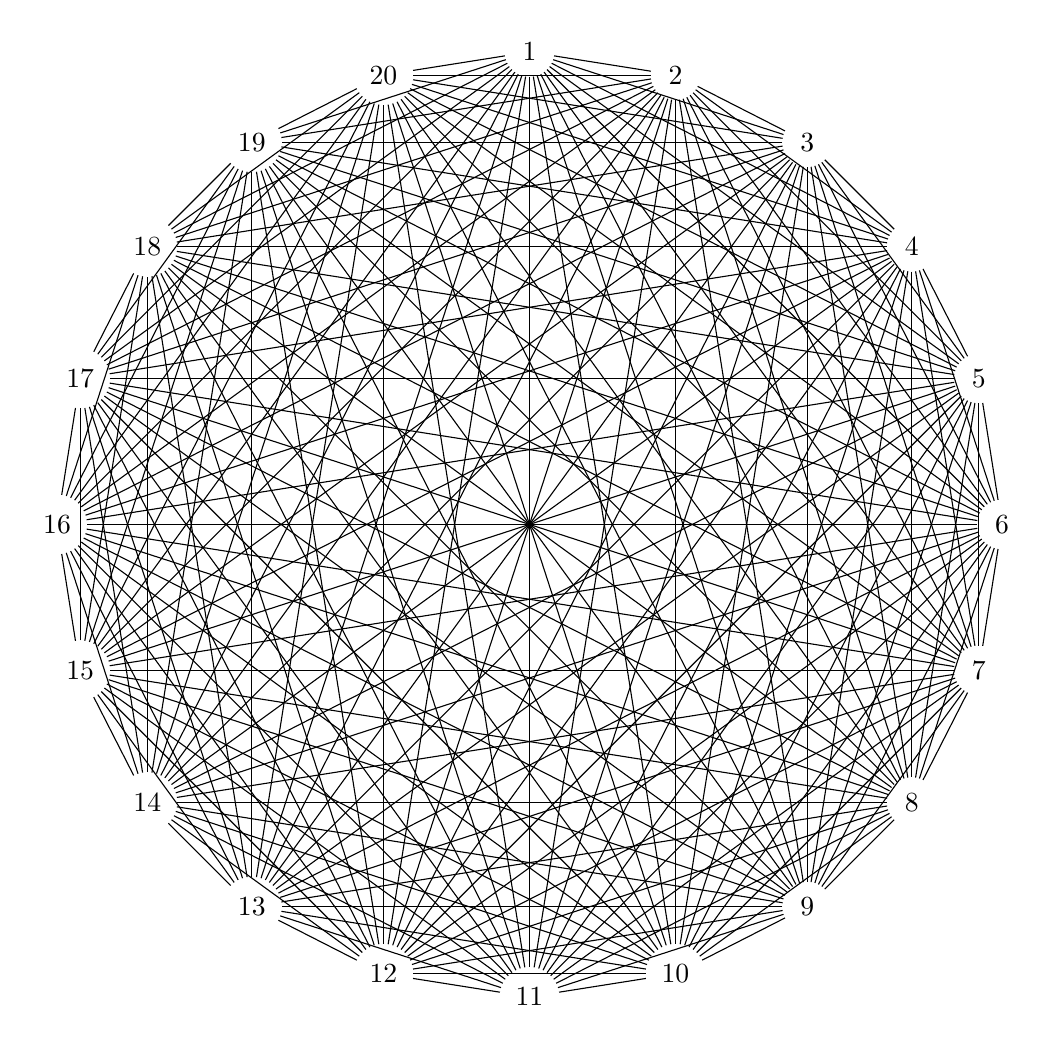
\begin{tikzpicture}[shape=circle]
    \graph { subgraph K_n [n=20,clockwise,radius=6cm] };
  \end{tikzpicture}
\caption{Graf predstavlja potrebne izmenjave šifrirnih ključev v primeru uporabe simetričnih šifrirnih algoritmov. Vsako vozlišče predstavlja enega uporabnika, povezave pa predstavljajo izmenjavo ključa med dvema uporabnikoma}
\label{fig:symmetricproblem}
\end{figure}

Ta problem lahko rešijo asimetrične šifre, ki uporabljajo en ključ za šifriranje, drug ključ pa dešifriranje. Tak par ključev imenujemo javni in zasebni ključ. Kot že ime pove, javni ključ ni nobena skrivnost in ga lahko brez skrbi objavimo na javnem mestu, obratno pa velja za zasebni ključ. Sporočilo, šifrirano z javnim ključem je možno dešifrirati samo s pripadajočim zasebnim ključem. Slabost asimetričnih šifer je njihova hitrost, saj z njimi ni praktično šifrirati večjih količin podatkov. Zato se v praksi največkrat uporabljajo protokoli, ki uporabljajo obe družini šifer, kot bomo videli kasneje.


\section{Simetrične šifre}

V kategorijo simetričnih šifer spadajo vse šifre, pri katerih se za šifriranje in dešifriranje uporablja enak ključ ali pa obstaja bijektivna preslikava, ki nam šifrirni ključ preslika v de-šifrirni in obratno. Simetrične šifre še naprej delimo na tokovne in bločne šifre. Poglavitna razlika med tokovnimi in bločnimi šiframi je v načinu šifriranja podatkov.

Naj bo dano sporočilo $X$ velikosti $n$ ($|X|=n$), ki je sestavljeno iz $n$ osnovnih nosilcev informacij (to so lahko biti, bajti ali kaj čisto tretjega). Simbol $\|$ predstavlja združevanje (lepljenje) dveh nizov.

$$
X=x_0 \| x_1 \| x_2 \| \dotsc \| x_{n-1}
$$

Bločna šifra vzame blok (del sporočila) velikosti $m$; $n=im, i\in\mathbb{N} $ in ga šifrira s ključem $K$. Tajnopis $Y$ tako pridobimo po naslednjem postopku:

\begin{gather*}
	y_j = e_K(e_{j} \| e_{j+1} \| \dotsc \| e_{j+m-1})  \quad j=0,1,\dotsc,i\\
	Y = y_0 \| y_1 \| \dotsc \| y_i
\end{gather*}

Bločne šifre delujejo na bloku podatkov fiksne velikosti (običajno velikost ključa določi velikost bloka) in v kolikor dolžina sporočila ni deljiva z $m$, je potrebno sporočilo dopolniti s posebnim zaporedjem znakov, dokler dolžina ni večkratnik števila $m$.

Drugačen pristop pa uporabljajo tokovne šifre, ki iz ključa $K$ ustvarijo neskončno zaporedje ključev $z$, ki ga nato uporabijo za šifriranje sporočila.

\begin{gather*}
z=z_0 \| z_1 \| z_2 \| \dotsc \| z_n \\
y_j=e_{z_j}(x_j) \quad j=0,1,\dotsc,n\\
Y = y_0 \| y_1 \| \dotsc \| y_n \\
\end{gather*}

Tak način šifriranja lahko uporabimo za poljubno dolga sporočila, brez potrebe po dopolnjevanju.

\newacronym{DES}{DES}{Data encryption standard}
\newacronym{NIST}{NIST}{National Institute of Standards and Technology}
\newacronym{NBS}{NBS}{National Bureau of Standards}


\newglossaryentry{feistelovasifra}
{
  name=Feistlova šifra,
  description={encryption key},
}

\subsection{DES in 3DES}

\gls{DES} je bil eden prvih modernih šifrirnih algoritmov. Originalna implementacija je nosila ime Lucifer in bila razvita v sedemdesetih letih v laboratorijih podjetja IBM.\  Kasneje je bila rahlo modificirana različica tega algoritma sprejeta s strani \acrshort{NIST}-a (takrat se je imenoval še \acrshort{NBS}) kot standard \gls{DES}.

\gls{DES} je simetrična bločna šifra, ki deluje na blokih velikosti 64 bitov in uporablja 64 bitni ključ, vendar je v ključu možno poljubno izbrati le 56 bitov, preostalih 8 pa se uporablja samo za odkrivanje napak v ključu.

Algoritem je sestavljen iz 16 identičnih korakov oziroma krogov, nekaj pre- in post-procesiranja vhodnih podatkov, Feistelove F-funkcije ter funkcije, ki iz glavnega ključa ustvari zaporedje podključev. Na začetku se 64-bitni blok razdeli na dve 32-bitni polovici, levo in desno, ki se po vsakem končanem krogu algoritma zamenjata. Taka shema delovanja je znana tudi kot \gls{feistelovasifra}. V vsakem krogu se leva polovica bloka z operacijo $XOR$ zmeša z rezultatom Feistelove F-funkcije, ki kot vhodne parametre dobi pod-ključ trenutnega kroga in desno polovico bloka. Po koncu vsakega kroga se leva in desna polovica zamenjata.

Ob prelomu tisočletja se je izkazalo da je \gls{DES}-ov 64-bitni o. 56-bitni ključ prešibak, da bi zadržal napade s surovo silo. Zato se je pojavila varianta algoritma imenovana 3DES.\ 3DES uporablja 3 ključe, pri čemer imamo na voljo 3 opcije za izbiro ključev.

\begin{enumerate}
\item Vse tri ključe izberemo neodvisno
\item Izberemo ključa $K_1$ in $K_2$ in $K_3=K_1$
\item Vsi ključi so isti, torej $K_1=K_2=K_3$
\end{enumerate}

Postopek šifriranja in dešifriranja je nato:

\begin{gather*}
C=E_{K_3}(D_{K_2}(E_{K_1}(P))) \\
P=D_{K_1}(E_{K_2}(D_{K_3}(C)))
\end{gather*}

Kjer je $C$ tajnopis in $P$ čistopis.

\newacronym{AES}{AES}{Advanced encryption standard}


\subsection{AES}

\gls{AES} je bil leta 2001 izbran kot naslednik standarda \gls{DES}. Med 15 prijavljenimi algoritmi je \gls{NIST} izbral družino algoritmov Rijndael. Kot standard \gls{AES} so bile sprejete tri različice algoritma. Vse tri uporabljajo 128-bitne bloke, razlikujejo pa se v velikosti ključa. Na voljo so 3 opcije: 128, 192 ali 256-bitni ključ.

\gls{AES} se po strukturi algoritma razlikuje od \gls{DES}-a, saj namesto Feistelove šifre uporablja substitucijsko-permutacijsko omrežje.  Algoritem iz ptičje perspektive izgleda tako:

\begin{description}
	\item[KeyExpansions] S posebnim algoritmom se na podlagi glavnega ključa izračunajo 128-bitni podključi, ki se bodo uporabili v vsakem krogu šifriranja.
	\item[AddRoundKey]  S pomočjo operacije $XOR$ se bloku čistopisa primeša 128-bitni pod-ključ.
	\item[SubBytes] Substitucija bajtov v bloku po pravilu ki ga določa S-škatla.
	\item[ShiftRows] Permutacija bajtov v bloku
	\item[MixColumns] Linearna transformacija
\end{description}

\begin{description}[style=nextline]
	\item[KeyExpansions]
	\item[Prvi krog]
		\begin{enumerate}
			\item AddRoundKey
		\end{enumerate}
	\item[Vmesni krogi]
		\begin{enumerate}
			\item SubBytes
			\item ShiftRows
			\item MixColumns
			\item AddRoundKey
		\end{enumerate}
	\item[Zadnji krogi]
		\begin{enumerate}
			\item SubBytes
			\item ShiftRows
			\item AddRoundKey
		\end{enumerate}

\end{description}

\newacronym{IV}{IV}{inicializacijski vektor}


\subsection{Načini delovanja bločnih šifer}

Bločna šifra sama po sebi kot vhodni podatek lahko sprejme samo blok točno določene dolžine, kar ni najbolj praktično, saj so sporočila pogosto različnih in predvsem nepredvidljivih velikosti. Poleg tega če isti blok čistopisa večkrat šifriramo z enakim ključem, dobimo kot rezultat vsakič isti tajnopis, kar je nezaželjen rezultat, saj morebitni napadalec lahko zazna vzorce v tajnopisu in iz tega poskuša razbrati pomen. Ta problem lahko rešimo tako, da uporabimo bločno šifro v enem od načinov delovanja.

Način delovanja je algoritem, ki pove kako vhodno sporočilo razdeliti na bloke primerne velikosti in na kak način na teh blokih potem uporabiti bločno šifro.

Večina načinov delovanja poleg bločne šifre in šifrirnega ključa potrebuje še \gls{IV}. Inicializacijski vektor skrbi, da tudi v primeru, da večkrat šifriramo isti čistopis z enakim ključem, dobimo kot rezultat različne tajnopise.

Kot smo že povedali, bločne šifre sprejemajo le bloke točno določene velikosti, zato je potrebno tudi v nekaterih načinih delovanja šifre sporočilo najprej dopolniti, tako da je njegova dolžina večkratnik velikosti bloka. Vendar obstajajo tudi načini delovanja, kjer to ni potrebno, saj ti iz bločne šifre naredijo tokovno šifro.

\newacronym{ECB}{ECB}{Electronic Codebook}

\subsubsection{ECB}
\label{subs:ECB}

Najpreprostejši način delovanja je \gls{ECB}. V tem načinu delovanja se sporočilo razdeli na bloke take velikosti, kot jih zahteva bločna šifra. Po potrebi se zadnji blok dopolni do zahtevane dolžine. Nato se vsak blok šifrira neodvisno od drugih, kar sicer pomeni da je možno operaciji šifriranja in dešifriranja na precej preprost način paralelizirati in s tem pohitriti. Prav tako je v tem načinu delovanja možno de-šifrirati poljubni blok sporočila, brez potrebe da najprej de-šifriramo vse predhodne bloke.

\begin{figure}[ht!]
  \centering
  \begin{subfigure}[b]{\textwidth}
    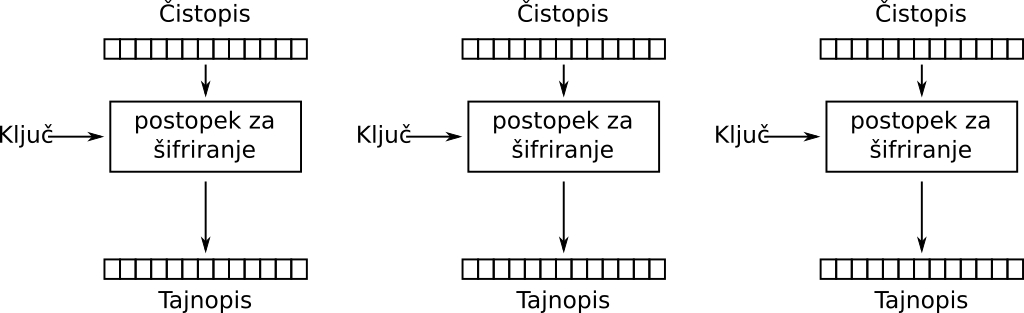
\includegraphics[width=\textwidth]{images/ECB_encryption}
    \caption{Šifriranje v načinu \gls{ECB}}
\label{fig:ecbenc}
  \end{subfigure}
  \begin{subfigure}[b]{\textwidth}
    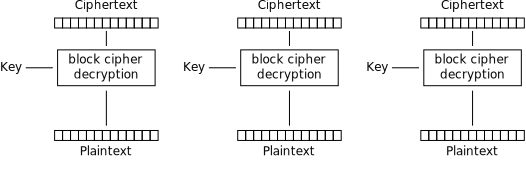
\includegraphics[width=\textwidth]{images/ECB_decryption}
    \caption{De-šifriranje v načinu \gls{ECB}}
\label{fig:ecbdec}
  \end{subfigure}
  \caption{Način delovanja \gls{ECB}}
\label{fig:ecbmode}

\end{figure}

Vse to so sicer dobrodošle lastnosti, vendar ima \gls{ECB} nekaj resnih pomanjkljivosti, zaradi katerih ni primeren za uporabo v resničnem svetu, ampak služi bolj kot opomin, da močni šifrirni algoritmi kot je \gls{AES}, ne zagotavljajo varnosti, če so uporabljeni na napačen način.

Slika~\ref{fig:ecbbad} prikazuje uporabo 128 bitne AES šifre v načinu ECB.\@ Na šifrirani sliki je še vedno možno razpoznati logotip Fakultete za računlništvo in informatiko, kar pomeni da tak način šifriranja ne zagotavlja varnosti.

\begin{figure}[ht!]
  \centering
  \begin{subfigure}[b]{0.3\textwidth}
    
\includegraphics[width=\textwidth]{images/LogoFRI}
    \caption{Original}
\label{fig:logoFRIorig}
  \end{subfigure}
  \begin{subfigure}[b]{0.3\textwidth}
    
\includegraphics[width=\textwidth]{images/LogoFRI_ecb}
    \caption{AES-128-ECB}
\label{fig:logoFRIECB}
  \end{subfigure}
  \begin{subfigure}[b]{0.3\textwidth}
    
\includegraphics[width=\textwidth]{images/LogoFRI_cbc}
    \caption{AES-128-CBC}
\label{fig:logoFRICBC}
  \end{subfigure}
  \caption{Primer različnih načinov šifriranja}
\label{fig:ecbbad}
\end{figure}

\newacronym{CBC}{CBC}{Cipher Block Chaining}

\subsubsection{CBC}
\label{subs:CBC}

V načinu \Gls{CBC} se vsak blok čistopisa pred šifriranjem s pomočjo operacije $XOR$ zmeša z tajnopisom prejšnjega bloka. Tak pristop naredi vsak naslednji blok odvisen od vseh prejšnjih blokov. S tem se rešimo problema ponavljajočih se vzorcev v tajnopisu, kot smo jih videli v načinu \acrshort{ECB} (slika~\ref{fig:ecbbad}). Posebni primer je prvi blok, saj tu nimamo na voljo tajnopisa prejšnjega bloka, s katerim bi izvedli operacijo $XOR$, zato namesto tajnopisa prejšnjega bloka uporabimo \acrfull{IV}. Dodatno nam naključni \gls{IV} doda tudi element naključnosti v tajnopis, kar pomeni da tudi če šifriramo enako sporočilo z enakim ključem, tajnopis ne bo enak, saj smo uporabili drugačen \gls{IV}.

Slabost takega pristopa pa je da je operacija šifriranja strogo zaporedna, saj naslednjega bloka ne moremo šifrirati dokler ne končamo šifriranja trenutnega bloka.

\begin{figure}[ht!]
  \centering
  \begin{subfigure}[b]{\textwidth}
    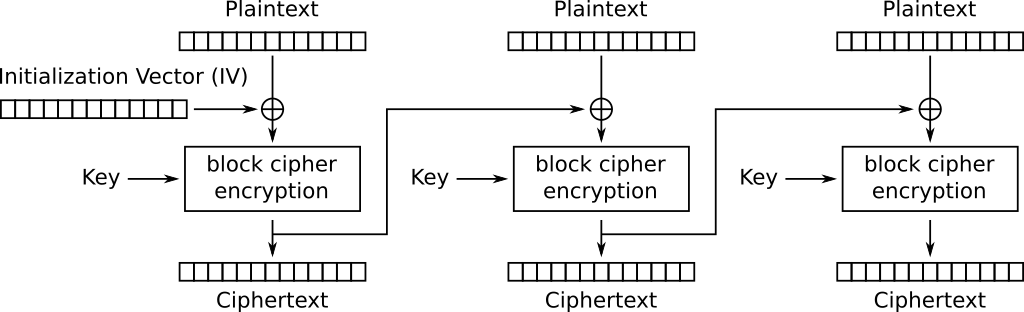
\includegraphics[width=\textwidth]{images/CBC_encryption}
    \caption{Šifriranje v načinu \gls{CBC}}
\label{fig:cbcenc}
  \end{subfigure}
  \begin{subfigure}[b]{\textwidth}
    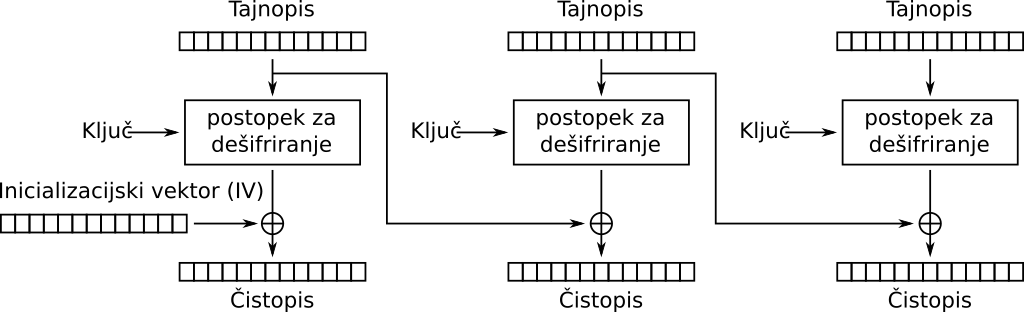
\includegraphics[width=\textwidth]{images/CBC_decryption}
    \caption{De-šifriranje v načinu \gls{CBC}}
\label{fig:cbcdec}
  \end{subfigure}
  \caption{Način delovanja \gls{CBC}}
\label{fig:cbcmode}
\end{figure}

\newacronym{CFB}{CFB}{Cipher Feedback}

\subsubsection{CFB}
\label{subs:CFB}

V \gls{CFB} načinu delovanja se bločna šifra uporablja kot tokovna. Prednost takega načina delovanja je, da ni potrebe po dopolnjevanju sporočila, prav tako pa se uporablja samo ena smer delovanja bločne šifre (to je ponavadi smer šifriranja), kar poenostavi implementacijo takega načina v strojni opremi.

Kot se vidi na sliki~\ref{fig:cfbmode}, se v tem načinu delovanja bločna šifra uporablja le za generiranje naključnega zaporedja, tajnopis pa rezultat operacije $XOR$ med čistopisom in naključnim zaporedjem, podobno kot pri enkratnem ščitu (angl.\ one time pad).

\begin{figure}[ht!]
  \centering
  \begin{subfigure}[b]{\textwidth}
    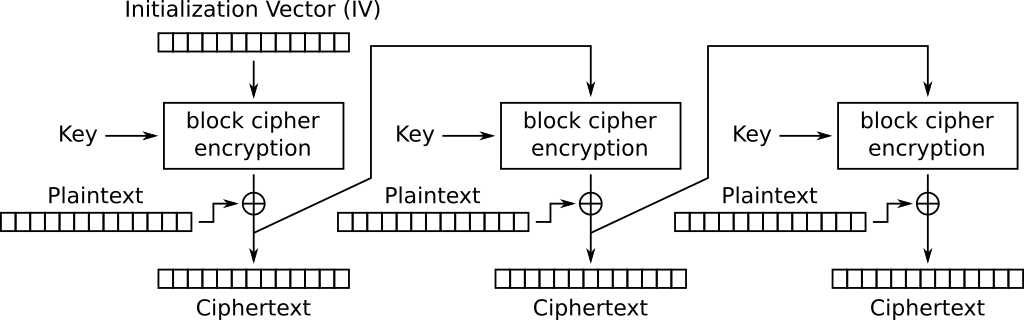
\includegraphics[width=\textwidth]{images/CFB_encryption}
    \caption{Šifriranje v načinu CFB}
\label{fig:cfbenc}
  \end{subfigure}
  \begin{subfigure}[b]{\textwidth}
    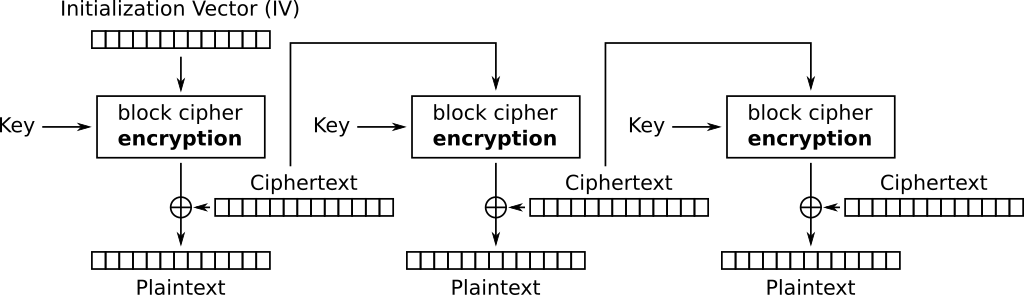
\includegraphics[width=\textwidth]{images/CFB_decryption}
    \caption{De-šifriranje v načinu CFB}
\label{fig:cfbdec}
  \end{subfigure}
  \caption{Način delovanja \gls{CFB}}
\label{fig:cfbmode}
\end{figure}

\newacronym{OFB}{OFB}{Output Feedback}


\subsubsection{OFB}
\label{subs:OFB}

V \gls{OFB} je podoben načinu \gls{CFB}, s to razliko, da se za generiranje naključnega zaporedja uporablja samo \gls{IV}. Prav to je lahko problematična lastnost, v primeru da šifriramo daljša sporočila, saj se lahko naredi cikel v naključnem zaporedju. To se lahko zgodi v primeru, da se v naključnem zaporedju pojavi blok, katerega tajnopis je enak IV.\@

\begin{figure}[ht!]
  \centering
  \begin{subfigure}[b]{\textwidth}
    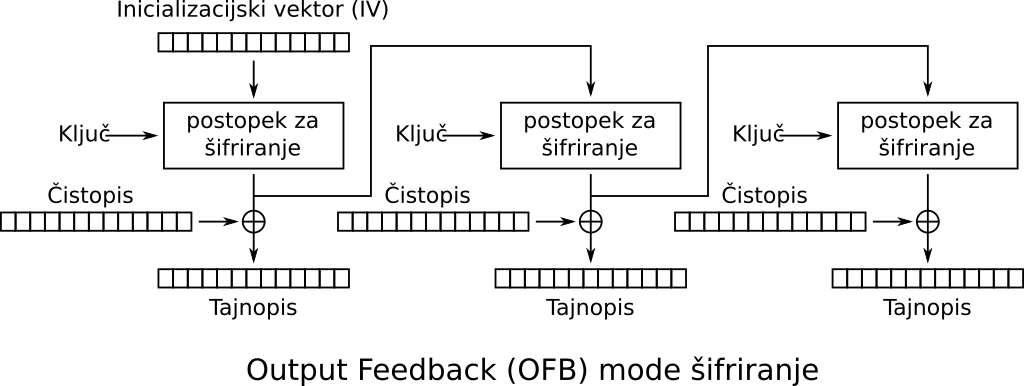
\includegraphics[width=\textwidth]{images/OFB_encryption}
    \caption{Šifriranje v načinu OFB}
\label{fig:ofbenc}
  \end{subfigure}
  \begin{subfigure}[b]{\textwidth}
    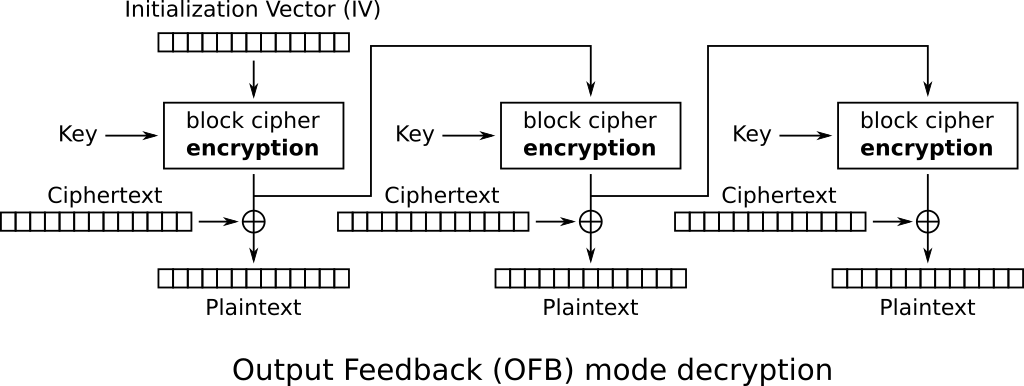
\includegraphics[width=\textwidth]{images/OFB_decryption}
    \caption{De-šifriranje v načinu OFB}
\label{fig:ofbdec}
  \end{subfigure}
  \caption{Način delovanja \gls{OFB}}
\label{fig:ofbmode}
\end{figure}



\section{Asimetrične šifre}

Eden večjih problemov simetričnih šifrirnih algoritmov je distribucija ključev. V kolikor želita dve osebi svojo komunikacijo zaščititi z uporabo simetričnega šifrirnega algoritma, se morata najprej izmenjati ključ. Dobra praksa je tudi, da se izognemo ponovni uporabi istega ključa, kar v praksi pomeni, da si moramo z vsako osebo, s katero želimo komunicirati izmenjati ključ in hitro se izkaže, da omrežje $n$ ljudi potrebuje $\frac{n(n-1)}{2}$ ključev. Če to preslikamo na omrežje kot je Internet, ki ga uporablja približno 40 odstotkov svetovne populacije. Vzemimo pesimistično oceno, da si vsak uporabnik Interneta lasti samo eno elektronsko napravo, ki uporablja varno komunikacijo in tako omrežje potrebuje $\approx 3.500.000.000$ izmenjav.

Rešitev za ta problem so lahko asimetrični šifrirni algoritmi, oziroma kriptografija javnih ključev. Asimetrični algoritmi ne uporabljajo samo enega, ampak dva ključa. Javni ključ poznajo vsi in ga uporabijo za šifriranje sporočil. Sporočila, šifrirana z javnim ključem, lahko dešifrira samo imetnik zasebnega ključa.

Asimetrični algoritmi delujejo na predpostavki, da so nekatere matematični v eno smer preprosto izračunljivi, v drugo pa preprosto pretežki, da bi jih bilo možno rešiti v razumnem časovnem okvirju. Eden takih problemov je faktorizacija števil. Če si izmislite dve dokaj veliki praštevili $p$ in $q$, ju med seboj pomnožite, dobite novo število $n$, za katero ni tako preprosto ugotoviti iz katerih faktorjev je sestavljeno, ob predpostavki, da ne poznamo $p$ in $q$.

Na žalost pa so zaradi svoje povezanosti s težkimi matematičnimi problemi pogosto asimetrični šifrirni algoritmi veliko počasnejši od svojih simetričnih sorodnikov. V praksi se uporablja kombinacija asimetričnih in simetričnih algoritmov. Asimetrični algoritmi so sicer počasnejši, vendar veliko bolj praktični zaradi preproste izmenjave ključev.

V začetni fazi vzpostavljanja varnega komunikacijska kanala se zaradi preprostejše distribucije ključev uporabi asimetrični algoritem. Ko je varni kanal vzpostavljen se preko njega izmenja sejni ključ, to je ključ ki se

\subsection{Izmenjava ključa Diffe-Hellman}
\label{sec:Izmenjava ključa Diffe-Hellman}


Metoda za izmenjavo ključa Diffe-Hellman je bil prvi javno objavljen algoritem, ki uporablja princip javnih in zasebnih ključev. V praksi omogoča, da se dva neznanca preko nezavarovanega kanala kot je Internet dogovorita za skupni ključ, ki ga bosta uporabljala za nadaljnjo komunikacijo. Prva sta ga objavila Whitfield Diffe in Martin Hellman leta 1976, vendar se je kasneje izkazalo, da je angleška tajna služba odkrila princip kriptografije javnih ključev že leto poprej, vendar to ostalo tajno do leta 1997.

Metoda temelji na reševanju problema diskretnega logaritma, za katerega matematiki verjamejo, da ne obstaja algoritem, ki ga bi bil sposoben rešiti v sprejemljivih časovnih okvirjih (izjema so algoritmi, ki tečejo na kvantnih računalnikih, vendar je to povsem drug svet).

Originalna različica algoritma uporablja multiplikativno grupo števil po modulu $p$, kjer je $p$ praštevilo in $g$ primitivni koren števila $p$.

Recimo da se želita Anita in Bojan preko Interneta dogovoriti o skupnem ključu, ki ga bosta uporabljala za nadaljnjo komunikacijo. To lahko storita po sledečem postopku:

\begin{mdframed}[frametitle={Izmenjava ključa Diffe-Hellman}]
\begin{enumerate}
	\item Anita in Bojan se dogovorita os skupnih parametrih, ki jih bosta uporabljala v algoritmu. To je praštevilo $p$ in primitivni koren praštevila $g$
	\item Anita si izbere skrivno število $a$, izračuna $A=g^a \mod p$ in pošlje $A$ Bojanu.
	\item Bojan si izbere skrivno število $b$, izračuna $B=g^b \mod p$ in pošlje $B$ Aniti.
	\item Anita izračuna $s=B^a \mod p$
	\item Bojan izračuna $s=A^b \mod p$
	\item Anita in Bojan sta dobila enak rezultat $s$, ki ga sedaj lahko uporabita kot skupni ključ za nadaljnjo komunikacijo.
\end{enumerate}

\vspace{0.5cm}

Oba sta izračunala enak rezultat, ker velja:
$$
A^b \equiv g^{ab} \equiv g^{ba} \equiv B^a \mod p
$$

\end{mdframed}

\newacronym{RSA}{RSA}{RSA}


\subsection{RSA}
\label{sub:RSA}

Medtem ko prej opisana metoda omogoča samo dogovor o skupnem ključu, pa je bil RSA prvi pravi kriptosistem, ki je uporabljal javne ključe. Varnost RSA temelji na tem, da je faktorizacija produkta dveh velikih praštevil težko rešljiv problem za današnje računalnike.

Javni ključ je par $(n, e)$, zasebni ključ pa par $(n, d)$, ki ju dobimo po naslednjem postopku:

\begin{enumerate}
\item Izberemo dve naključni, približno enako veliki praštevili $p$ in $q$
\item Izračunamo $n=pq$
\item Izračunamo $\varphi(n)=\varphi(p)\varphi(q)=(p-1)(q-1)$
\item Izberemo število $e$, tako da $1<e<\varphi(n)$ tako da je $e$ tuje $\varphi(n)$
\item Izračunamo $d$, tako da $d \equiv e^{-1} \pmod{\varphi(n)}$
\end{enumerate}

Poleg zasebnega ključa moramo moramo paziti tudi na zasebnost vrednosti $p$, $q$ in $\varphi(n)$

\todo{napisi vec}

\subsection{Šifriranje na osnovi pogojev}
\label{subs:Šifriranje na osnovi pogojev}
\newacronym{IBE}{IBE}{Identity Based Encryption}
\newacronym{ABE}{ABE}{Attribute Based Encryption}
\newacronym{KP-ABE}{KP-ABE}{Key-policy attribute based encryption}
\newacronym{CP-ABE}{CP-ABE}{Ciphertext-policy attribute based encryption}

Šifriranje na osnovi pogojev je eden najnovših pristopov na področju kriptografije javnih ključev. V tradicionalni kriptografski shemi javnih ključev se sporočilo šifrira za točno določenega prejemnika (tistega, kateremu pripada javni ključ, ki ga uporabimo za šifriranje). Korak dlje je šlo šifriranje na osnovi identitete (angl. \acrlong{IBE}), kjer lahko za javni ključ uporabimo kar preprost niz znakov, kot je recimo prejemnikov e-naslov. Šifriranje na osnovi pogojev pa je šlo še korak dlje, saj dovoljuje, da isti tajnopis dešifria kdorkoli poseduje ključ, ki zadovolji vse pogoje.

Poglejmo si za primer Anito, ki shrani šifrirane podatke v oblak. Anita ima datoteko $X$, ki bi jo rada delila s skupinama $Prijatelji$ in $Znanci$. Prav tako ima datoteko $Y$, ki bi jo rada delila s skupinama $Družina$ in $Prijatelji$. To lahko stori tako, da ustvari en ključ za datoteko $X$ in ta ključ deli s $Prijatelji$ in $Znanci$, nato ustvari drug ključ za datoteko $Y$ in ta ključ deli s skupinama $Družina$ in $Prijatelji$. Problem je, da mora Anita za vsako datoteko, ki jo želi deliti, ustvariti nov ključ.

Naivna rešitev tega problema bi bila, da Anita ustvari en ključ za vsako skupino ljudi, s katerimi želi deliti datoteke. Vendar življenje ni preprosto, in lahko se zgodi, da neka oseba pripada večim skupinam s katerimi želi Anita deliti datoteke. Prav tako si lahko zaželi deliti neko datoteko samo z ljudmi, ki so hkrati $Prijatelji$ in $Sodelavci$. Recimo da je to datoteka $Z$. Tako datoteko lahko najprej šifrira s ključem, ki pripada skupini $Prijatelji$ in nato še s ključem, ki pripada skupini $Sodelavci$. Naivno bi mislili da je to dobra rešitev, vendar se izkaže da tak sistem ni odporen proti zaroti. Šifrirano datoteko lahko kot posamezniki odprejo samo ljudje, ki pripadajo obema skupinama, saj imajo le oni v posesti oba ključa. Vendar pa se lahko proti Aniti zarotita dva posameznika skupaj, kjer noben od nju ne pripada obema skupinama hkrati, vendar imata skupaj dostop do obeh ključev, saj vsak od nju pripada eni od skupin.

Možnost dešifriranja določajo pravila, ki so predstavljena z drevesi, kjer so notranja vozlišča logične operacije, listi pa pogoji, ki so lahko zadovoljeni ali nezadovoljeni. Drevo beremo od listov proti korenu in za vsako notranje vozlišče ugotovimo ali je v zadovoljenem ali nezadovoljenem stanju. Na koncu pridemo do korena drevesa, in dešifriranje uspe samo v primeru, da je koren drevesa v zadovoljenem stanju.

Poznamo dve vrsti šifriranja na osnovi parametrov. V prvem je drevo, ki določa pravila shranjeno v ključu  (angl. \acrlong{KP-ABE}), v drugem primeru pa je shranjeno v tajnopisu (angl. \acrlong{CP-ABE}).

\section{Homomorfne šifre}
\label{subs:Homomorfne šifre}

Šifre, o katerih smo katerih smo govorili do sedaj, imajo to lastnost da je njihov tajnopis kolikor je pač možno naključen.

\chapter{Uporaba kriptografije v oblaku}

Največji problem uporabe šifriranja v oblaku je v bistvu enak kot povsod kjer poskušamo zagotoviti varnost na tak in drugačen način. Potrebno je najti kompromis med zadovoljivim nivojem varnosti in uporabnostjo. Trivialno je narediti 100\% varen sistem, vendar ta verjetno ne bo kaj prida uporaben.

Prav tako ločimo tri stanja digitalnih podatkov: podatki v mirovanju, podatki v gibanju in podatki v uporabi. V vsakem stanju obstajajo različne varnostne zahteve, zato se potrebni različni pristopi. Jaber in Zolkipli\cite{jaber2013use} sta uporabila tabelo~\ref{tbl:cloudtriad}, ki lepo ponazori načine uporabe kriptografije glede na različna stanja podatkov.

\begin{table}[]
  \centering
  \begin{tabular}{lllll}
                                        & Podatki v mirovanju                   & Podatki v uporabi                    & Podatki v gibanju              &  \\ \cline{2-4}
    \multicolumn{1}{l|}{Zaupnost}       & \multicolumn{1}{l|}{Simetrične šifre} & \multicolumn{1}{l|}{Homomorfne šifre} & \multicolumn{1}{l|}{TLS}        &  \\ \cline{2-4}
    \multicolumn{1}{l|}{Istovetnost}    & \multicolumn{1}{l|}{MAC}              & \multicolumn{1}{l|}{Homomorfne šifre} & \multicolumn{1}{l|}{TLS}        &  \\ \cline{2-4}
    \multicolumn{1}{l|}{Razpoložjivost} & \multicolumn{1}{l|}{redundanca}       & \multicolumn{1}{l|}{redundanca}       & \multicolumn{1}{l|}{redundanca} &  \\ \cline{2-4}
  \end{tabular}
  \caption{}
\label{tbl:cloudtriad}
\end{table}

Zgodovinsko gledano je bila kriptografija izumljena z motivom varovanja komunikacij, torej podatkov v gibanju, vendar na problem varovanja podatkov v mirovanju lahko gledamo kot na komunikacijo s samim sabo. To nam predvsem poenostavi problem distribucije ključev, zato so za varovanje podatkov v mirovanju zelo primerne simetrične šifre.

Na začetku obdobja računalništva se največ pozornosti posvečalo predvsem varnosti podatkov v mirovanju, saj so se informacijski sistemi nahajali znotraj podjetja, oziroma so bili do podjetja povezani preko najetih vodov. Prav tako so se podatki obdelovali na strojni opremi, ki je bila v lasti podjetja in se je nahajala na varni lokaciji. S prihodom storitev v oblaku, se je ta paradigma spremenila. Podatke je treba najprej prenesti v oblačni sistem, največkrat kar preko Interneta. Prav tako podatke v oblak pošljemo z namenom, da jih bomo tam obdelovali in analizirali, kar pomeni da je potrebno poskrbeti tudi za varnost podatkov v uporabi.

\newacronym{SSL}{SSL}{Secure Sockets Layer}
\newacronym{TLS}{TLS}{Transport Layer Security}

To se odraža tudi v pristopih k varovanju podatkov v različnih stanjih. Dočim za varovanje podatkov v mirovanju obstajajo ustaljene prakse, pa za ostali dve področji velja, da se nenehno spreminjata. Na področju varovanja podatkov v gibanju, ki ga v primeru oblačnih sistemov večinoma pokrivata kriptografska protokola \acrfull{SSL} in njegov naslednik \acrfull{TLS}, je v zadnjih letih prišlo do odkritji različnih napadov in posledično opustitve določenih verzij protokolov, ker te niso več zagotavljale zadovoljivega nivoja varnosti. Drugačna pa je situacija na področju varovanja podatkov v uporabi, saj v preteklosti ni bilo velike potrebe po praktični implementaciji takih kriptografskih protokolov, vendar se je s prihodom oblačnih storitev tudi to področje začelo pospešeno razvijati.


\newglossaryentry{cold-boot-attack}
{
  name=Cold boot attack,
  description={Cold boot attack},
}

\newglossaryentry{deduplication}
{
  name=izločanje dvojnic,
  description={angl.\ deduplication},
}

\section{Varovanje podatkov v mirovanju}
\label{subs:Varovanje podatkov v mirovanju}

Podatke v mirovanju predstavljajo vsi podatki na trajnem pomnilniku, izključujoč podatke ki so trenutno v gibanju in podatke, ki so trenutno v delovnem pomnilniku računalnika. Praviloma so to podatki ki se ne spreminjajo pogosto oziroma arhivski podatki, ki se sploh ne spreminjajo. Količinsko predstavljajo glavnino vseh podatkov, kar pomeni da morajo biti kriptografski algoritmi, ki delujejo na temi podatki hitri. Zato se za varovanje takih podatkov zelo primerne simetrične šifre.

Podatki v mirovanju so dolgotrajne narave, kar pomeni da je dolgotrajna tudi skrb za varnost šifrirnih ključev, ki nam zagotavljajo dostop do teh podatkov. V preteklosti so bili ključi ``shranjeni'' kar v uporabnikovi glavi, vendar ob količini podatkov s katerimi operiramo danes, je to žal postala misija nemogoče. Dodaten problem predstavlja dejstvo, da je do podatkov pogosto potreben povsem avtomatski dostop, brez posredovanja človeka.

V kontekstu oblačnih sistemov je pri zagotavljanju varnosti podatkov v mirovanju najbolj problematičen del prav upravljanje s ključi, saj je potrebno poskrbeti za ključe velikega števila uporabnikov. Prav tako je s stališča varnosti neodgovorno, da zaupamo ustvarjanje in upravljanje šifrirnih ključev tretji osebi, v našem primeru ponudniku storitve v oblaku. Zato je v primeru, da je potrebno zagotoviti visoko stopnjo varnosti, kljub temu pa želimo podatke hraniti v oblaku, najbolj primerna šifriranje podatkov še preden jih pošljemo v oblak, tako imenovano client-side šifriranje. Prednosti so očitne, saj šifrirni ključ nikoli ne rabi zapustiti našega računalnika, tako da smo lahko prepričani, da do naših podatkov shranjenih v oblaku, ne more dostopati nihče.

V primeru oblačnih storitev, ki ponujajo hrambo velikih količin podatkov v oblaku (storitve, kot so Dropbox) pa je zaželena lastnost tudi sposobnost \glslink{deduplication}{izločanja dvojnic}. Kot smo omenili v poglavju~\ref{sec:Kaj je oblak?}, oblačni sistemi izkoriščajo skupno rabo sredstev, kar pomeni da so datoteke večjega števila uporabnikov shranjene na skupnem pomnilniku. Pogosto se namreč zgodi, da več uporabnikov želi shraniti identično datoteko v oblak in v takem primeru je najbolj optimalna rešitev da se taka datoteka shrani samo enkrat, saj bi v nasprotnem primeru samo tratili razpoložljiv prostor z podvojenimi kopijami datotek. Vendar v primeru uporabe šifriranja se bo ista datoteka, šifrirana s ključi dveh različnih uporabnikov zelo verjetno zašifrirala v dva popolnoma različna tajnopisa.

% \begin{mdframed}[frametitle={Semantična varnost}]
% Kriptosistem je semantično varen, če iz tajnopisa ni mogoče na praktičen način\footnote{v polinomskem času na verjetnostnem Turingovem stroju} pridobiti nobene informacije o čistopisu.
% \end{mdframed}

\subsubsection{Šifrirni algoritmi}
\label{subs:Šifrirni algoritmi}
\todo{}

\subsubsection{Upravljanje ključev}
\label{subs:Upravljanje ključev}
\todo{}

\subsubsection{Konvergentne kriptografske sheme}
\label{subs:Konvergentne kriptografske sheme}


\begin{mdframed}[frametitle={Polinomska varnost}]
\label{def:polysec}
Za dano šifrirno funkcijo $e$ in poljubna dva čistopisa $p_1$ in $p_2$ iz katerih pridobimo tajnopisa $c=e(p_1)$ in $c=e(p_1)$ velja: Sistem je polinomsko varen, če velja da v polinomskem času ne moremo ugotoviti kateri $c$ pripada kateremu čistopisu z verjetnostjo občutno večjo kot $0.5$.
\end{mdframed}


\newglossaryentry{ciphertext indistinguishability}
{
  name=ciphertext indistinguishability,
  description={angl.\ ciphertext indistinguishability},
}

Kasneje sta~\cite{Goldwasser1984} Goldwasser in Micali pokazala, da je problem semantične varnosti enakovreden problemu \gls{ciphertext indistinguishability}, ki zahteva, da napadalec ne more razločiti poljubnih dveh tajnopisov glede na njun čistopis.

The primary security disadvantage of this approach, as identified
in its original description [10], is that it leaks some information. In
particular, convergent encryption reveals if two ciphertext strings
decrypt to the same plaintext value. However, this behavior is nec-
essary in systems that use deduplication, since it allows a system
to remove duplicate plaintext data chunks while only observing the
ciphertext; information leakage is part of the compromise needed
to achieve space-efficiency through deduplication.

Problem izločanja dvojnic in zagotavljanja (semantične) varnosti


\section{Varovanje podatkov v gibanju}
\label{sec:Varovanje podatkov v gibanju}

Za podatke v gibanju veljajo vsi podatki, ki se preko interneta pretakajo od uporabnika proti oblaku in obratno. Poleg tega pa so podatki v gibanju tudi vsi podatki, ki se prenašajo med različnimi strežniki znotraj oblačnega sistema.

Omrežja po katerih podatki potujejo velikokrat uporabljajo dinamične usmerjevalne algoritme, ne moremo vnaprej vedeti po kateri poti bodo podatki potovali. Podatki v gibanju na svoji poti potujejo skozi veliko omrežnih naprav, katere imajo vse vpogled v podatke, prav tako pa jim ne moremo zaupati. Dodatno nevarnost predstavlja še napad \gls{MITM}, kjer napadalec izkoristi dinamičnost omrežja in se vrine na pot podatkov med uporabnika in oblačni sistem.

Podatki so v gibanju praviloma malo časa, zato ni potrebe po kompleksnem upravljanju ključev. S pomočjo algoritmov za varno izmenjavo ključev, kot je recimo Diffe-Hellman algoritem opisan v poglavju~\ref{sec:Izmenjava ključa Diffe-Hellman}, je možno da se za vsako sejo uporabi nov, naključno generiran ključ.

% Najbolj razširjen protokol za zaščito podatkov med tem ko so v gibanju je \gls{SSL} in njegov naslednik \gls{TLS}. Poleg njega se predvsem za statične povezave med dvema omrežjema uporabljajo še protokoli iz družine VPN. Znotraj omrežja ponudnika pa se lahko uporabijo tudi tehnologije kot je VLAN. VLAN ne zagotavlja varnosti s pomočjo šifriranja, ampak deluje na principu omejevanja dostopa do prometa, ki sicer poteka po skupnem mediju. Tak način pristopa sicer ščiti pred napadalci, ki imajo ustrezno malo pooblastil, recimo drugi uporabniki sistema, ne more pa nas začititi pred napadalci notranjimi napadalci, kot so zaposleni pri ponudniku storitve.

\subsection{SSL in TLS}
\label{sub:SSL in TLS}
\todo[inline]{Opis protokola, opis napadov}

\subsubsection{Prihodnja varnost}
\label{subs:Prihodnja varnost}



\section{Varovanje podatkov v uporabi}
\label{sec:Varovanje podatkov v uporabi}

\newglossaryentry{rootkit}
{
  name=korenski komplet,
  description={angl.\ rootkit},
}

\newglossaryentry{varno vecstransko racunanje}
{
  name=varno večstransko računanje,
  description={angl.\ secure multi-party computation},
}

Podatki v uporabi so zelo kratkotrajne narave, vendar jih je kljub temu zelo težko zaščititi. Problem izhaja iz same definicije podatkov v uporabi, saj so to podatki, nad katerimi računalniški sistem želi izvesti neko operacijo, oziroma jih prikazati uporabniku. Podatki v uporabi se nahajajo v delovnem pomnilniku računalnika, in so zato izpostavljeni tako imenovanemu \glslink{cold-boot-attack}{napadu cold-boot}, kjer napadalec dobesedno zamrzne stanje pomnilnika ob delujočem računalniku in nato poskuša iz njega izvleči vsebino, predvsem šifrirne ključe, saj lahko z njihovo pomočjo dešifrira veliko večjo količino podatkov, ki so trenutno v mirovanju ali gibanju.

Kjub temu pa tveganje za napad cold-boot ni veliko, saj z napadalčeve strani zahteva fizičen dostop do sistema in kar nekaj tehnologije. Večji problem predstavlja morebitna okužba sistema s \glslink{rootkit}{korenskim kompletom}, ki napadalcu omogoča dostop do celotnega pomnilnika sistema.

V nadaljevanju bomo predstavili tri možnih načinov, kako zagotoviti različne stopnje zasebnosti podatkov v uporabi.

\subsubsection{Varno večstransko računanje}
\label{subs:Varno večstransko računanje}

Varno večstransko računanje je področje kriptografije, ki se ukvarja z razvojem algoritmov, ki omogočajo, da več udeležencev skupaj izračuna rezultat neke funkcije, brez da bi kdorkoli poznal vse vhodne parametre funkcije.


\todo[inline]{Šifriranje delovnega pomnilnika, homomorfna enkricpija, secure MPC, ...}



\newpage

%********************************************

\addcontentsline{toc}{chapter}{Seznam slik}
\addtocontents{toc}{\protect\vspace{-2ex}}
\listoffigures

\newpage

\addcontentsline{toc}{chapter}{Seznam tabel}
\listoftables

%\listofalgorithms


%********************************************

\newpage
\nocite{*}
\bibliographystyle{slplainurl}
\addcontentsline{toc}{chapter}{Literatura}
\label{literatura}
\bibliography{diploma}

\end{document}
